\documentclass[12pt,a4paper]{article}
\usepackage[utf8]{inputenc} %polskie znaki
\usepackage[T1]{fontenc}	%polskie znaki
\usepackage{amsmath}		%matematyczne znaczki :3
\usepackage{enumerate}		%Dodatkowe opcje do funkcji enumerate
\usepackage{geometry} 		%Ustawianie marginesow
\usepackage{graphicx}		%Grafika
\usepackage{wrapfig}		%Grafika obok textu
\usepackage{float}			%Allows H in fugire
\usepackage{xcolor}     	% for colour
\usepackage{lipsum}     	% for sample text
\usepackage{ntheorem}   	% for theorem-like environments
\usepackage{mdframed}   	% for framing
%\usepackage{amsthm}		%Dodaje przerwa u góry w twierdzeniach
%\pagestyle{empty} 			%usuwa nr strony

\theoremstyle{break}
\theoreminframepreskip{0.5cm}
\theoremheaderfont{\bfseries}
\newmdtheoremenv[%
linecolor=white,%
innertopmargin=\topskip,
shadowsize=0,%
innertopmargin=5,%
innerbottommargin=5,%
leftmargin=10,%
rightmargin=10,%
backgroundcolor=gray!20,%
innertopmargin=0pt,%
ntheorem]{zad}{Zadanie}


\newgeometry{tmargin=2cm, bmargin=2cm, lmargin=2cm, rmargin=2cm} 

\begin{document}
	
	\begin{center}
		\LARGE Wielomiany, funkcje wykładnicze i logarytmiczne - test
	\end{center}
	
	\begin{tabular}{p{13cm} r}
		Imię i nazwisko: ............................................................................
		&[....../40pkt]\\ 
		\vspace{0.5cm}
	\end{tabular}
	
	\begin{zad}[0-3]
		\textbf{Zapisz poniższe wyrażenia w postaci} $a^x$ \textbf{.}
	\end{zad} 
	
	\begin{enumerate}[a)]\Large
		\item $\frac{5^5\cdot(5^2)^5}{(5^{-4})^6}=$
		\item $\frac{5^{15}\cdot25^7}{125^6}=$
		\item $\frac{14^{12}\cdot8^3}{49^6}=$
	\end{enumerate}
	
	%%%%%%%%%%%%%%%%%%%%%%%%%%%%%
	
	\begin{zad}[0-1]
		\textbf{Dokończ zdanie. Wybierz właściwą odpowiedź spośród podanych.}
	\end{zad} 
	
	Połowa liczby \Large$\frac{4^{60}\;\cdot\;4^{-50}}{4^{-10}}\:$\normalsize wynosi:
	
	\vspace{0.5cm}
	\begin{tabular}{p{3.5cm} p{3.5cm} p{3.5cm} p{3.5cm}}
		\textbf{A. }$2^{10}$&
		\textbf{B. }$4^{10}$&
		\textbf{C. }$2^{20}$&
		\textbf{D. }$2^{19}$\\
	\end{tabular}
	
	%%%%%%%%%%%%%%%%%%%%%%%%%%%%%
	
	\begin{zad}[0-3]
		\textbf{Wykaż, że liczba:}
		$$k=2^{2023}+2^{2024}$$
		\textbf{jest podzielna przez 6.}
	\end{zad} 
	
	
	\begin{tabular}{|p{0.1cm}|p{0.1cm}|p{0.1cm}|p{0.1cm}|p{0.1cm}|p{0.1cm}|p{0.1cm}|p{0.1cm}|p{0.1cm}|p{0.1cm}|p{0.1cm}|p{0.1cm}|p{0.1cm}|p{0.1cm}|p{0.1cm}|p{0.1cm}|p{0.1cm}|p{0.1cm}|p{0.1cm}|p{0.1cm}|p{0.1cm}|p{0.1cm}|p{0.1cm}|p{0.1cm}|p{0.1cm}|p{0.1cm}|p{0.1cm}|p{0.1cm}|p{0.1cm}|p{0.1cm}|p{0.1cm}|p{0.1cm}}
		\hline&&&&&&&&&&&&&&&&&&&&&&&&&&&&&&\\
		\hline&&&&&&&&&&&&&&&&&&&&&&&&&&&&&&\\
		\hline&&&&&&&&&&&&&&&&&&&&&&&&&&&&&&\\
		\hline&&&&&&&&&&&&&&&&&&&&&&&&&&&&&&\\
		\hline&&&&&&&&&&&&&&&&&&&&&&&&&&&&&&\\
		\hline&&&&&&&&&&&&&&&&&&&&&&&&&&&&&&\\
		\hline&&&&&&&&&&&&&&&&&&&&&&&&&&&&&&\\
		\hline&&&&&&&&&&&&&&&&&&&&&&&&&&&&&&\\
		\hline&&&&&&&&&&&&&&&&&&&&&&&&&&&&&&\\
		\hline&&&&&&&&&&&&&&&&&&&&&&&&&&&&&&\\
		\hline&&&&&&&&&&&&&&&&&&&&&&&&&&&&&&\\
		\hline&&&&&&&&&&&&&&&&&&&&&&&&&&&&&&\\
		\hline&&&&&&&&&&&&&&&&&&&&&&&&&&&&&&\\
		\hline&&&&&&&&&&&&&&&&&&&&&&&&&&&&&&\\
		\hline&&&&&&&&&&&&&&&&&&&&&&&&&&&&&&\\
		\hline&&&&&&&&&&&&&&&&&&&&&&&&&&&&&&\\
		\hline&&&&&&&&&&&&&&&&&&&&&&&&&&&&&&\\
		\hline
	\end{tabular}
	
	
	
	\newpage
	%%%%%%%%%%%%%%%%%%%%%%%%%%%%%
	
	\begin{mdframed}[%
		linecolor=white,%
		innertopmargin=\topskip,
		shadowsize=0,%
		innertopmargin=5,%
		innerbottommargin=5,%
		leftmargin=10,%
		rightmargin=10,%
		backgroundcolor=gray!20,%
		innertopmargin=0pt,]
		\vspace{0.2cm}
		\textbf{\textit{Informacja do zadań 4-5.}}
		
		
	\end{mdframed}
	
	Poniżej przedstawiono wykres funkcji wykładniczej, której wzór wyraża się w postaci $$f(x)=a^x.$$
	
	\begin{figure}[h]
		\centering
		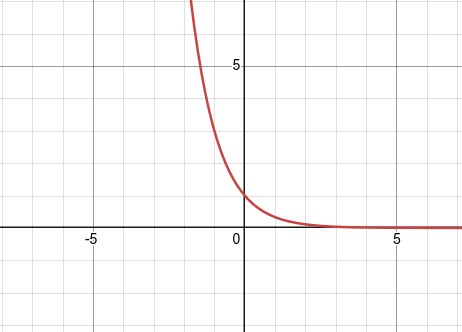
\includegraphics[scale=0.7]{wifw.jpeg}
	\end{figure}
	
	%%%%%%%%%%%%%%%%%%%%%%%%%%%%%
	
	\begin{zad}[0-1]
		\textbf{Dokończ zdanie. Wybierz właściwą odpowiedź spośród podanych.}
	\end{zad} 
	
	Wartość wyrażenia $f(-f(0))$ jest równa:
	
	\vspace{0.5cm}
	\begin{tabular}{p{3.5cm} p{3.5cm} p{3.5cm} p{3.5cm}}
		\textbf{A. }$-3$&
		\textbf{B. }$0$&
		\textbf{C. }$1$&
		\textbf{D. }$3$\\
	\end{tabular}
	
	%%%%%%%%%%%%%%%%%%%%%%%%%%%%%
	
	\begin{zad}[0-3]
		\textbf{Wyznacz współczynnik "a" powyższej funkcji wykładniczej.}
	\end{zad} 
	
	\begin{tabular}{|p{0.1cm}|p{0.1cm}|p{0.1cm}|p{0.1cm}|p{0.1cm}|p{0.1cm}|p{0.1cm}|p{0.1cm}|p{0.1cm}|p{0.1cm}|p{0.1cm}|p{0.1cm}|p{0.1cm}|p{0.1cm}|p{0.1cm}|p{0.1cm}|p{0.1cm}|p{0.1cm}|p{0.1cm}|p{0.1cm}|p{0.1cm}|p{0.1cm}|p{0.1cm}|p{0.1cm}|p{0.1cm}|p{0.1cm}|p{0.1cm}|p{0.1cm}|p{0.1cm}|p{0.1cm}|p{0.1cm}|p{0.1cm}}
		\hline&&&&&&&&&&&&&&&&&&&&&&&&&&&&&&\\
		\hline&&&&&&&&&&&&&&&&&&&&&&&&&&&&&&\\
		\hline&&&&&&&&&&&&&&&&&&&&&&&&&&&&&&\\
		\hline&&&&&&&&&&&&&&&&&&&&&&&&&&&&&&\\
		\hline&&&&&&&&&&&&&&&&&&&&&&&&&&&&&&\\
		\hline&&&&&&&&&&&&&&&&&&&&&&&&&&&&&&\\
		\hline&&&&&&&&&&&&&&&&&&&&&&&&&&&&&&\\
		\hline&&&&&&&&&&&&&&&&&&&&&&&&&&&&&&\\
		\hline&&&&&&&&&&&&&&&&&&&&&&&&&&&&&&\\
		\hline&&&&&&&&&&&&&&&&&&&&&&&&&&&&&&\\
		\hline&&&&&&&&&&&&&&&&&&&&&&&&&&&&&&\\
		\hline&&&&&&&&&&&&&&&&&&&&&&&&&&&&&&\\
		\hline&&&&&&&&&&&&&&&&&&&&&&&&&&&&&&\\
		\hline&&&&&&&&&&&&&&&&&&&&&&&&&&&&&&\\
		\hline&&&&&&&&&&&&&&&&&&&&&&&&&&&&&&\\
		\hline
	\end{tabular}
	
	\newpage
	%%%%%%%%%%%%%%%%%%%%%%%%%%%%%
	
	\begin{zad}[0-1]
		\textbf{Dokończ zdanie. Wybierz właściwą odpowiedź spośród podanych.}
	\end{zad} 
	
	Wyrażenie $\sqrt[5]{9\sqrt{3}}$ można zapisać w postaci:
	
	\vspace{0.5cm}
	\begin{tabular}{p{3.5cm} p{3.5cm} p{3.5cm} p{3.5cm}}
		\textbf{A. }$\sqrt[7]{27}$&
		\textbf{B. }$\sqrt[10]{3}$&
		\textbf{C. }$\sqrt{3}$&
		\textbf{D. }$\sqrt[10]{27}$\\
	\end{tabular}	
	
	%%%%%%%%%%%%%%%%%%%%%%%%%%%%%
	
	\begin{zad}[0-2]
		\textbf{Oblicz:}
	\end{zad} 
	
	\begin{enumerate}[a)]
		\item $\sqrt{11}+\sqrt{99}+\sqrt{121}=$
		\item $4\sqrt{45}-3\sqrt{125}+2\sqrt{500}=$
	\end{enumerate}
	
	%%%%%%%%%%%%%%%%%%%%%%%%%%%%%
	
	\begin{zad}[0-1]
		\textbf{Dokończ zdanie. Wybierz właściwą odpowiedź spośród podanych.}
	\end{zad} 
	
	Wartość wyrażenia $\log_3(\frac{1}{9})$ wynosi:
	
	\vspace{0.5cm}
	\begin{tabular}{p{3.5cm} p{3.5cm} p{3.5cm} p{3.5cm}}
		\textbf{A. }$-3$&
		\textbf{B. }$-\frac{1}{3}$&
		\textbf{C. }$\frac{1}{3}$&
		\textbf{D. }$-2$\\
	\end{tabular}
	
	%%%%%%%%%%%%%%%%%%%%%%%%%%%%%
	
	\begin{zad}[0-4]
		\textbf{Oblicz:}
	\end{zad} 
	
	\begin{enumerate}[a)]
		\item $2\log0,001=$
		\item $\log_2(\log_749^8)=$
		\item $\log_51000-3\log_52=$
		\item $\log_5625+\log_48=$
	\end{enumerate}
	
	%%%%%%%%%%%%%%%%%%%%%%%%%%%%%
	
	\begin{zad}[0-1]
		\textbf{Dokończ zdanie. Wybierz właściwą odpowiedź spośród podanych.}
	\end{zad} 
	
	Wyrażenie $\log_{\sqrt{2}}16$ jest równe:
	
	\vspace{0.5cm}
	\begin{tabular}{p{3.5cm} p{3.5cm} p{3.5cm} p{3.5cm}}
		\textbf{A. }$-4$&
		\textbf{B. }$4$&
		\textbf{C. }$8$&
		\textbf{D. }$16$\\
	\end{tabular}

	\newpage
	%%%%%%%%%%%%%%%%%%%%%%%%%%%%%

	\begin{zad}[0-5]
		\textbf{Rozwiąż równanie}
		$$x^6-12x^4-64x^2=0$$
	\end{zad} 
	
	\begin{tabular}{|p{0.1cm}|p{0.1cm}|p{0.1cm}|p{0.1cm}|p{0.1cm}|p{0.1cm}|p{0.1cm}|p{0.1cm}|p{0.1cm}|p{0.1cm}|p{0.1cm}|p{0.1cm}|p{0.1cm}|p{0.1cm}|p{0.1cm}|p{0.1cm}|p{0.1cm}|p{0.1cm}|p{0.1cm}|p{0.1cm}|p{0.1cm}|p{0.1cm}|p{0.1cm}|p{0.1cm}|p{0.1cm}|p{0.1cm}|p{0.1cm}|p{0.1cm}|p{0.1cm}|p{0.1cm}|p{0.1cm}|p{0.1cm}}
		\hline&&&&&&&&&&&&&&&&&&&&&&&&&&&&&&\\
		\hline&&&&&&&&&&&&&&&&&&&&&&&&&&&&&&\\
		\hline&&&&&&&&&&&&&&&&&&&&&&&&&&&&&&\\
		\hline&&&&&&&&&&&&&&&&&&&&&&&&&&&&&&\\
		\hline&&&&&&&&&&&&&&&&&&&&&&&&&&&&&&\\
		\hline&&&&&&&&&&&&&&&&&&&&&&&&&&&&&&\\
		\hline&&&&&&&&&&&&&&&&&&&&&&&&&&&&&&\\
		\hline&&&&&&&&&&&&&&&&&&&&&&&&&&&&&&\\
		\hline&&&&&&&&&&&&&&&&&&&&&&&&&&&&&&\\
		\hline&&&&&&&&&&&&&&&&&&&&&&&&&&&&&&\\
		\hline&&&&&&&&&&&&&&&&&&&&&&&&&&&&&&\\
		\hline&&&&&&&&&&&&&&&&&&&&&&&&&&&&&&\\
		\hline&&&&&&&&&&&&&&&&&&&&&&&&&&&&&&\\
		\hline&&&&&&&&&&&&&&&&&&&&&&&&&&&&&&\\
		\hline&&&&&&&&&&&&&&&&&&&&&&&&&&&&&&\\
		\hline
	\end{tabular}
	
	%%%%%%%%%%%%%%%%%%%%%%%%%%%%%

	\begin{zad}[0-5]
		\textbf{Rozwiąż równanie}
		$$2x^3-2x^2=16x-16$$
	\end{zad} 
	
	\begin{tabular}{|p{0.1cm}|p{0.1cm}|p{0.1cm}|p{0.1cm}|p{0.1cm}|p{0.1cm}|p{0.1cm}|p{0.1cm}|p{0.1cm}|p{0.1cm}|p{0.1cm}|p{0.1cm}|p{0.1cm}|p{0.1cm}|p{0.1cm}|p{0.1cm}|p{0.1cm}|p{0.1cm}|p{0.1cm}|p{0.1cm}|p{0.1cm}|p{0.1cm}|p{0.1cm}|p{0.1cm}|p{0.1cm}|p{0.1cm}|p{0.1cm}|p{0.1cm}|p{0.1cm}|p{0.1cm}|p{0.1cm}|p{0.1cm}}
		\hline&&&&&&&&&&&&&&&&&&&&&&&&&&&&&&\\
		\hline&&&&&&&&&&&&&&&&&&&&&&&&&&&&&&\\
		\hline&&&&&&&&&&&&&&&&&&&&&&&&&&&&&&\\
		\hline&&&&&&&&&&&&&&&&&&&&&&&&&&&&&&\\
		\hline&&&&&&&&&&&&&&&&&&&&&&&&&&&&&&\\
		\hline&&&&&&&&&&&&&&&&&&&&&&&&&&&&&&\\
		\hline&&&&&&&&&&&&&&&&&&&&&&&&&&&&&&\\
		\hline&&&&&&&&&&&&&&&&&&&&&&&&&&&&&&\\
		\hline&&&&&&&&&&&&&&&&&&&&&&&&&&&&&&\\
		\hline&&&&&&&&&&&&&&&&&&&&&&&&&&&&&&\\
		\hline&&&&&&&&&&&&&&&&&&&&&&&&&&&&&&\\
		\hline&&&&&&&&&&&&&&&&&&&&&&&&&&&&&&\\
		\hline&&&&&&&&&&&&&&&&&&&&&&&&&&&&&&\\
		\hline&&&&&&&&&&&&&&&&&&&&&&&&&&&&&&\\
		\hline&&&&&&&&&&&&&&&&&&&&&&&&&&&&&&\\
		\hline
	\end{tabular}

	\newpage
	%%%%%%%%%%%%%%%%%%%%%%%%%%%%%
	
	\begin{zad}[0-5]
		\textbf{Rozwiąż równanie}
		$$\frac{x^2-x-6}{x^2+2x-15}=0$$
	\end{zad} 
	
	\begin{tabular}{|p{0.1cm}|p{0.1cm}|p{0.1cm}|p{0.1cm}|p{0.1cm}|p{0.1cm}|p{0.1cm}|p{0.1cm}|p{0.1cm}|p{0.1cm}|p{0.1cm}|p{0.1cm}|p{0.1cm}|p{0.1cm}|p{0.1cm}|p{0.1cm}|p{0.1cm}|p{0.1cm}|p{0.1cm}|p{0.1cm}|p{0.1cm}|p{0.1cm}|p{0.1cm}|p{0.1cm}|p{0.1cm}|p{0.1cm}|p{0.1cm}|p{0.1cm}|p{0.1cm}|p{0.1cm}|p{0.1cm}|p{0.1cm}}
		\hline&&&&&&&&&&&&&&&&&&&&&&&&&&&&&&\\
		\hline&&&&&&&&&&&&&&&&&&&&&&&&&&&&&&\\
		\hline&&&&&&&&&&&&&&&&&&&&&&&&&&&&&&\\
		\hline&&&&&&&&&&&&&&&&&&&&&&&&&&&&&&\\
		\hline&&&&&&&&&&&&&&&&&&&&&&&&&&&&&&\\
		\hline&&&&&&&&&&&&&&&&&&&&&&&&&&&&&&\\
		\hline&&&&&&&&&&&&&&&&&&&&&&&&&&&&&&\\
		\hline&&&&&&&&&&&&&&&&&&&&&&&&&&&&&&\\
		\hline&&&&&&&&&&&&&&&&&&&&&&&&&&&&&&\\
		\hline&&&&&&&&&&&&&&&&&&&&&&&&&&&&&&\\
		\hline&&&&&&&&&&&&&&&&&&&&&&&&&&&&&&\\
		\hline&&&&&&&&&&&&&&&&&&&&&&&&&&&&&&\\
		\hline&&&&&&&&&&&&&&&&&&&&&&&&&&&&&&\\
		\hline&&&&&&&&&&&&&&&&&&&&&&&&&&&&&&\\
		\hline&&&&&&&&&&&&&&&&&&&&&&&&&&&&&&\\
		\hline
	\end{tabular}
	
	%%%%%%%%%%%%%%%%%%%%%%%%%%%%%
	
	\begin{zad}[0-5]
		\textbf{Uprość wyrażenie}
		$$\frac{3x^2-15x}{6x^2-42x+60}:\frac{x^3+4x}{x^2-4x+4}=$$
	\end{zad} 
	
	\begin{tabular}{|p{0.1cm}|p{0.1cm}|p{0.1cm}|p{0.1cm}|p{0.1cm}|p{0.1cm}|p{0.1cm}|p{0.1cm}|p{0.1cm}|p{0.1cm}|p{0.1cm}|p{0.1cm}|p{0.1cm}|p{0.1cm}|p{0.1cm}|p{0.1cm}|p{0.1cm}|p{0.1cm}|p{0.1cm}|p{0.1cm}|p{0.1cm}|p{0.1cm}|p{0.1cm}|p{0.1cm}|p{0.1cm}|p{0.1cm}|p{0.1cm}|p{0.1cm}|p{0.1cm}|p{0.1cm}|p{0.1cm}|p{0.1cm}}
		\hline&&&&&&&&&&&&&&&&&&&&&&&&&&&&&&\\
		\hline&&&&&&&&&&&&&&&&&&&&&&&&&&&&&&\\
		\hline&&&&&&&&&&&&&&&&&&&&&&&&&&&&&&\\
		\hline&&&&&&&&&&&&&&&&&&&&&&&&&&&&&&\\
		\hline&&&&&&&&&&&&&&&&&&&&&&&&&&&&&&\\
		\hline&&&&&&&&&&&&&&&&&&&&&&&&&&&&&&\\
		\hline&&&&&&&&&&&&&&&&&&&&&&&&&&&&&&\\
		\hline&&&&&&&&&&&&&&&&&&&&&&&&&&&&&&\\
		\hline&&&&&&&&&&&&&&&&&&&&&&&&&&&&&&\\
		\hline&&&&&&&&&&&&&&&&&&&&&&&&&&&&&&\\
		\hline&&&&&&&&&&&&&&&&&&&&&&&&&&&&&&\\
		\hline&&&&&&&&&&&&&&&&&&&&&&&&&&&&&&\\
		\hline&&&&&&&&&&&&&&&&&&&&&&&&&&&&&&\\
		\hline&&&&&&&&&&&&&&&&&&&&&&&&&&&&&&\\
		\hline&&&&&&&&&&&&&&&&&&&&&&&&&&&&&&\\
		\hline
	\end{tabular}


	
\end{document}